\vspace{-.2cm}
\section{Experiments}
\vspace{-.2cm}
In this section, we comprehensively evaluate the performance of PH-Reg on a diverse set of dense tasks, first using a zero-shot setup for open-vocabulary segmentation in section~\ref{section_seg}, followed by linear probe based segmentation and depth tasks in section~\ref{section_linear}. Finally we perform ablation studies to explore design decisions and investigate the nature of artifacts across different models in section~\ref{section_ablation}.
All implementation details are provided in the appendix. 

% Please add the following required packages to your document preamble:
% \usepackage{graphicx}
\renewcommand{\arraystretch}{1.2}
\begin{table*}[t!]
\centering
\caption{\textbf{Open-vocabulary Semantic Segmentation Quantitative Evaluation Results on 8 Benchmarks.} While the first 3 benchmarks (VOC21, PC60 and Obejct) include a background class, the remaining benchmarks do not. We report the mean Intersection over Union (mIoU, \%) metric, where higher values indicate better performance, for our method and all baseline models. The best result for each dataset is highlighted in \textbf{bolded}. Additional results are provided in the supplementary material.}
\vspace{.1cm}
\resizebox{1.0\columnwidth}{!}{%
\begin{tabular}{l|ccccccccc}
\hline
Method         & VOC21 & PC60 & Object & VOC20 & PC59 & Stuff & City & ADE & Avg.  \\ \hline
CLIP~\citep{Radford2021LearningTV}           & 18.60  & 7.84      & 6.50         & 49.05 & 11.17     & 7.19       & 6.65      & 3.16   & 13.77 \\
MaskCLIP~\citep{zhou2022extract}       & 49.27 & 25.46     & 26.94       & 66.56 & 28.62     & 18.80       & 28.33     & 13.70   & 32.21 \\
SCLIP~\citep{wang2024scliprethinkingselfattentiondense}          & 59.62 & 31.74     & 33.52       & 81.53 & 34.46     & 22.65      & 32.34     & 16.45  & 40.08 \\
ClearCLIP~\citep{lan2024clearclip}      & 59.76 & 32.56     & 32.77       & \textbf{84.56} & 35.91     & 23.89      & 30.04     & 16.65  & 39.52 \\
NACLIP~\citep{hajimiri2025naclip}         & 58.88 & 32.20      & 33.15       & 79.70  & 35.16     & 23.30       & 35.48     & 17.42  & 39.41 \\ \hline
MaskCLIP + DVT~\citep{zhou2022extract,yang2024denoising} & 44.29 & 25.08     & 20.89       & 65.88 & 29.50      & 17.10       & 30.89     & 14.06  & 30.96 \\
NACLIP + DVT~\citep{hajimiri2025naclip, yang2024denoising}   & 60.25 & 32.73     & 32.89       & 80.26 & 35.91     & 23.41      & 36.31     & 17.54  & 39.91 \\
Ours (PH-Reg)  & \textbf{63.01} & \textbf{34.52}     & \textbf{35.27}       & 83.05 & \textbf{37.88}     & \textbf{24.66}      & \textbf{37.17}     & \textbf{19.22}  & \textbf{41.85} \\ \hline
\end{tabular}%
}
\vspace{-.2cm}
\label{tab:ovss}
\end{table*}


\vspace{-.2cm}
\subsection{Open-vocabulary Semantic Segmentation Evaluation}
\label{section_seg}
\vspace{-.2cm}

\textbf{Datasets.} In this section, we follow prior works \citep{wang2024scliprethinkingselfattentiondense,hajimiri2025naclip,lan2024clearclip} to evaluate our approach on six semantic segmentation datasets, with their names abbreviated (in parentheses) to conserve table space: PASCAL VOC 2012 (VOC21)~\citep{everingham2015pascal}, PASCAL Context (PC 60)~\citep{context}, COCO-Object (Object)~\citep{cocoobjects}, COCO-Stuff (Stuff)~\citep{caesar2018coco}, Cityscape (City)~\citep{cordts2016cityscapes}, ADE20K-150 (ADE)~\citep{ade20k}. In addition to these standard benchmarks, we also evaluate on two commonly used variants, PASCAL VOC 2012 (VOC20) and PASCAL Context (PC 59), in which the background class is excluded from the evaluation. 
For all experiments, we utilize the same evaluation harness for all methods, and apply a sliding window inference strategy for non-square images. We also resize input images such that the shorter side is fixed to specific resolutions, accommodating the varying original image sizes across datasets. 

\textbf{Baselines.} We compare our method against several relevant approaches in open-vocabulary semantic segmentation, including MaskCLIP~\citep{zhou2022extract}, SCLIP~\citep{wang2024scliprethinkingselfattentiondense}, ClearCLIP~\citep{lan2024clearclip}, and NACLIP~\citep{hajimiri2025naclip}. We also include vanilla CLIP as a baseline in our comparison, as it can be adapted for semantic segmentation. Unless otherwise specified, all visual encoders use the widely adopted pretrained ViT backbone with the same \texttt{OpenAI CLIP ViT-B/16} weights to ensure a fair comparison. We also include denoised versions of MaskCLIP and NACLIP produced by DVT, as DVT represents a closely related method to our approach. Unless otherwise noted, for CLIP we adopt the most basic MaskCLIP framework (direct \textit{v} output without any attention modifications) as our student model.
Notably, we re-implemented all baselines using the same prompt templates as in ~\cite{wang2024scliprethinkingselfattentiondense, hajimiri2025naclip}. All reported results are obtained without any post-processing refinement. 

\textbf{Quantitative Results.} Table~\ref{tab:ovss} summarizes the quantitative comparison results of various open-vocabulary semantic segmentation models. We observe that PH-Reg CLIP consistently outperforms all compared methods on 7 out of 8 evaluated benchmarks, with particularly strong results in VOC21 (63.01\%) and COCO Object (35.27\%). Moreover, PH-Reg CLIP surpasses the denoised versions of MaskCLIP and NACLIP, where DVT fails to yield significant performance gains. We believe this is caused by the residual estimator in DVT, which assumes stationary artifacts -- an assumption that does not hold consistently for training-free open vocabulary segmentation methods based CLIP. We note that ClearCLIP slightly outperforms our method on the VOC20 dataset. This may be attributed to its use of correlative self-attention, \emph{i.e.} \emph{q-q} attention, which incorporates feature localization cues. This explanation is plausible, as SCLIP, which also employs \emph{q-q} attention, similarly outperforms NACLIP on the VOC20 dataset.

\textbf{Qualitative Results.} Figure~\ref{fig:local} presents a qualitative comparison between our PH-Reg CLIP and three baseline models: MaskCLIP, SCLIP, and NACLIP. We visualize the UMAP of the dense features produced by each model, as well as the corresponding heatmaps generated from different text queries.
Our qualitative observations are as follows:
\textbf{1.} Artifact tokens are frequently observed in the UMAP visualizations of MaskCLIP, SCLIP, and NACLIP. While some artifact tokens are reduced in the heatmap of MaskCLIP, they remain prevalent in the heatmaps of both SCLIP and NACLIP.
\textbf{2.} The presence of artifact tokens hinders the models' ability to maintain fine-grained spatial alignment with the text queries, leading to suboptimal localization.
\textbf{3.} In contrast, PH-Reg CLIP consistently produces cleaner UMAPs and more fine-grained, semantically aligned heatmaps, which correspond well to meaningful local image structures.
These visualizations demonstrate that our method effectively preserves the consistency of dense feature representations and enhances semantic alignment between visual and textual modalities.

\vspace{-.2cm}
\subsection{Linear Probe Based Segmentation \& Depth Evaluation}\label{section_linear}
\vspace{-.2cm}
\textbf{Datasets \& Baselines.} In this section, we evaluate our approach in two semantic segmentation datasets: PASCAL VOC 2012 (VOC21)~\cite{everingham2015pascal} and ADE20K-150 (ADE)~\cite{ade20k} and one monocular depth estimation dataset: NYUv2-Depth dataset (NYUd)~\cite{silberman2012nyu}.
Since DVT~\cite{yang2024denoising} targets a similar objective with our approach, we include both the vanilla models and their denoised versions produced by DVT as comparison baselines.
We adopt the same linear probe experimental setup as in~\citep{yang2024denoising}, and train a linear layer integrated into the backbones, as a decode head to predict pixel-wise segmentation or depth logits from patch tokens.
Table~\ref{tab:linear} summarizes the main experiment results.

% Please add the following required packages to your document preamble:
% \usepackage{multirow}
% \usepackage{graphicx}
\renewcommand{\arraystretch}{1.2}
\begin{table*}[t!]
\centering
\caption{\textbf{Linear Probe Based Evaluation Results on Segmentation and Depth.} PH-Reg improves pretrained ViT backbones across various dense prediction tasks. For semantic segmentation, we report the mean Intersection over Union (mIoU, \%) metric and mean accuracy (mAcc, \%). For monocular depth estimation, we report Root Mean Squared Error (RMSE), absolute relative error (Abs Rel), and accuracy under threshold $\delta_1$. The best result for each dataset is highlighted in \textbf{bold}.}
\vspace{.1cm}
\resizebox{0.95\columnwidth}{!}{%
\begin{tabular}{l|cc|cc|ccc}
\hline
\multirow{2}{*}{Method} & \multicolumn{2}{c|}{VOC21}       & \multicolumn{2}{c|}{ADE}         & \multicolumn{3}{c}{NYUd}                            \\
                        & mIoU($\uparrow$)           & mAcc($\uparrow$)           & mIoU($\uparrow$)           & mAcc($\uparrow$)           & RMSE($\downarrow$)            & Abs Rel($\downarrow$)         & $\delta_{1}$($\uparrow$)              \\ \hline
CLIP~\citep{Radford2021LearningTV}                    & 73.88          & 83.37          & 35.78          & 47.3           & 0.6843          & 0.2115          & 64.93          \\
CLIP + DVT~\citep{Radford2021LearningTV,yang2024denoising}                & 74.74          & 84.33          & 36.39          & 48.14          & 0.6800             & 0.2089              & 65.07               \\
NACLIP~\citep{hajimiri2025naclip}                  & 74.01          & 83.16          & 37.06          & 48.33          & 0.6852          & 0.2082          & 64.52          \\
NACLIP + DVT~\citep{hajimiri2025naclip,yang2024denoising}              & 74.47          & 82.98          & 36.91          & 48.56          & 0.6845          & 0.2122          & 65.11          \\
MaskCLIP~\citep{zhou2022extract}                & 70.28          & 79.06          & 34.43          & 44.74          & \textbf{0.6645}          & 0.2030          & 67.71          \\
MaskCLIP + DVT~\citep{zhou2022extract,yang2024denoising}            & 71.38          & 80.49          & 34.43          & 44.86          & 0.6792          & 0.2091          & 64.96          \\
Ours (PH-Reg)           & \textbf{75.32} & \textbf{84.96} & \textbf{38.07} & \textbf{49.58} & 0.6746 & \textbf{0.1995} & \textbf{68.17} \\ \hline
OpenCLIP~\citep{ilharco_gabriel_2021_5143773}                & 71.31          & 80.64          & 37.68          & 49.8           & 0.6853          & 0.2113          & 64.86          \\
OpenCLIP + DVT~\citep{ilharco_gabriel_2021_5143773,yang2024denoising}             & 72.58          & 83.42          & 38.30          & 50.91          & 0.6811          & 0.2159          & 64.73          \\
OpenCLIP + Ours           & \textbf{73.25} & \textbf{83.99} & \textbf{39.32} & \textbf{51.24} & \textbf{0.6784} & \textbf{0.2019} & \textbf{65.32} \\ \hline
DFN-CLIP~\citep{fang2023data}                & 71.98          & 82.07          & 36.81          & 47.83          & 0.6860          & 0.2118          & 64.50          \\
DFN-CLIP + DVT~\citep{fang2023data, yang2024denoising}            & \textbf{73.09}          & \textbf{83.52}         & 37.73          & 49.39          & 0.6852          & 0.2092          & 64.65          \\
DFN-CLIP + Ours           & 72.97 & 82.48 & \textbf{39.15} & \textbf{50.61} & \textbf{0.6768} & \textbf{0.2052} & \textbf{65.26} \\ \hline
DINOv2~\cite{oquab2023dinov2}                  & 84.13          & 92.00             & 47.82          & 60.50           & 0.4566          & 0.1391          & 82.92          \\
DINOv2 + DVT~\citep{oquab2023dinov2,yang2024denoising}              & \textbf{85.43}         & \textbf{93.37}          & \textbf{48.86}          & \textbf{61.61}          & 0.4329          & 0.1289          & 85.23          \\
DINOv2 + Ours            & 84.85 & 92.46 & 48.66 & 61.57 & \textbf{0.4306} & \textbf{0.1216} & \textbf{86.35} \\ \hline
\end{tabular}%
}
\vspace{-.2cm}
\label{tab:linear}
\end{table*}

\textbf{Semantic Segmentation Results.}  As shown in Table~\ref{tab:linear}, We observe significant and consistent improvements, outperforming at least 4 out of 6 denoised ViT backbones across the evaluated datasets. 
While DVT consistently enhances the performance of DINOv2 and vanilla CLIP, it provides only limited improvements for other ViT backbones derived from other CLIP models. 
In contrast, our approach yields substantial performance boosts across these backbones, especially a notable +5.04\% mIoU on VOC21 and +3.64\% mIoU on ADE20k. These results demonstrate that our method can be robustly adopted to enhance the performance of diverse ViT backbones in semantic segmentation.

Notably, DVT relies on neural fields and requires gradient-based optimization, making the iterative denoising process applied to each image individually highly time-consuming. Our method leverages test-time augmentation for denoising, enabling the generation of cleaner dense feature representations without incurring excessive computational overhead. However, our results also show that the residual estimator as introduced in DVT may be beneficial to some model types (DINOv2, DFN-CLIP) more so than others. These results highlight that PH-Reg achieves superior performance in suppressing artifact tokens through a more robust and efficient design.

\textbf{Depth Estimation Results.}  Following prior work~\citep{oquab2023dinov2,yang2024denoising} we adopt AdaBins~\citep{Bhat2021adabins} for monocular depth evaluation. 
As shown in Table~\ref{tab:linear}, our method consistently improves the performance of pretrained ViT backbones whereas the DVT assumption of stationary artifacts mostly hold true for DINOv2. Additionally, DVT achieves performance gains using an additional transformer block with 0.08× the parameters of the base models~\citep{yang2024denoising}, our method achieves superior results with only a negligible increase in parameter count introduced by the register tokens.
These results demonstrate the efficiency of our approach, yielding noticeable performance gains with minimal model overhead.

\subsection{Ablation Studies and Investigation of Artifacts}
\label{section_ablation}
\vspace{-.2cm}
In this section, we conduct ablation studies on \texttt{OpenAI CLIP ViT-B/16} to investigate  various architectural and training components, focusing on both model performance and training feasibility.
\begin{figure}[h!]
  \centering
    \begin{subfigure}[t]{0.58\linewidth}
    \centering
    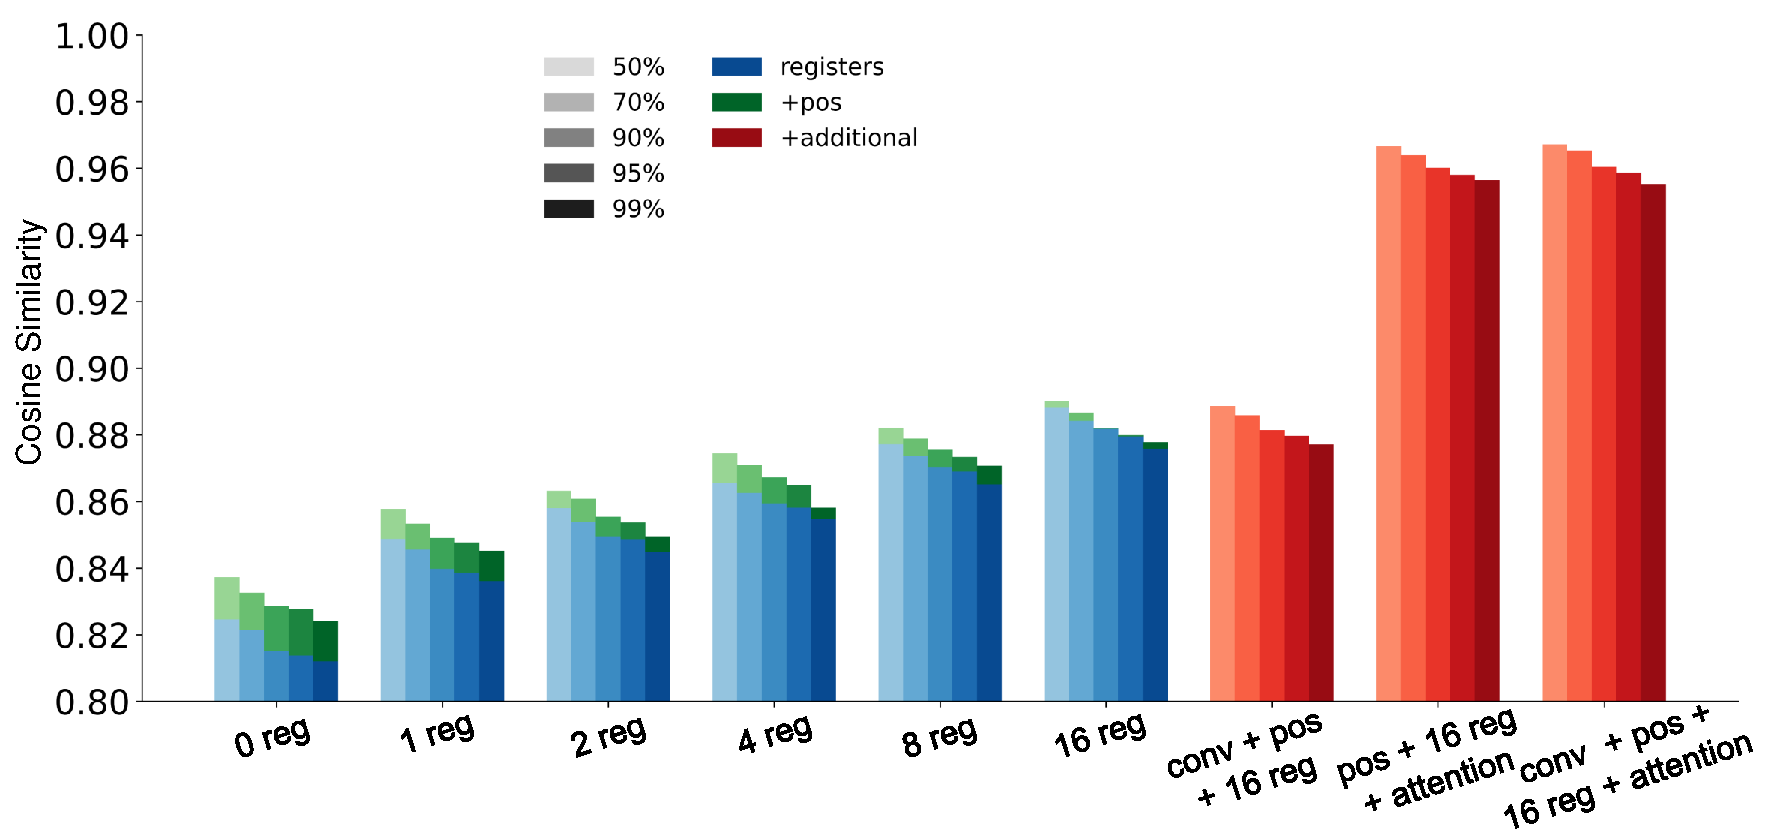
\includegraphics[width=0.98\linewidth]{fig_pdf/ablation_reg_layers_123_cropped.pdf}
    \caption{\textbf{Registers' behavior.} This plot illustrates adding registers improve PH-Reg teacher performance. In the blue settings, only registers are unfreezed. The green settings represent the improvements when positional embeddings are unlocked additionally. The red settings represent performance of unlocking more layers.}
    \label{fig:ablation_reg}
  \end{subfigure}
  \hfill
  \begin{subfigure}[t]{0.38\linewidth}
    \centering
    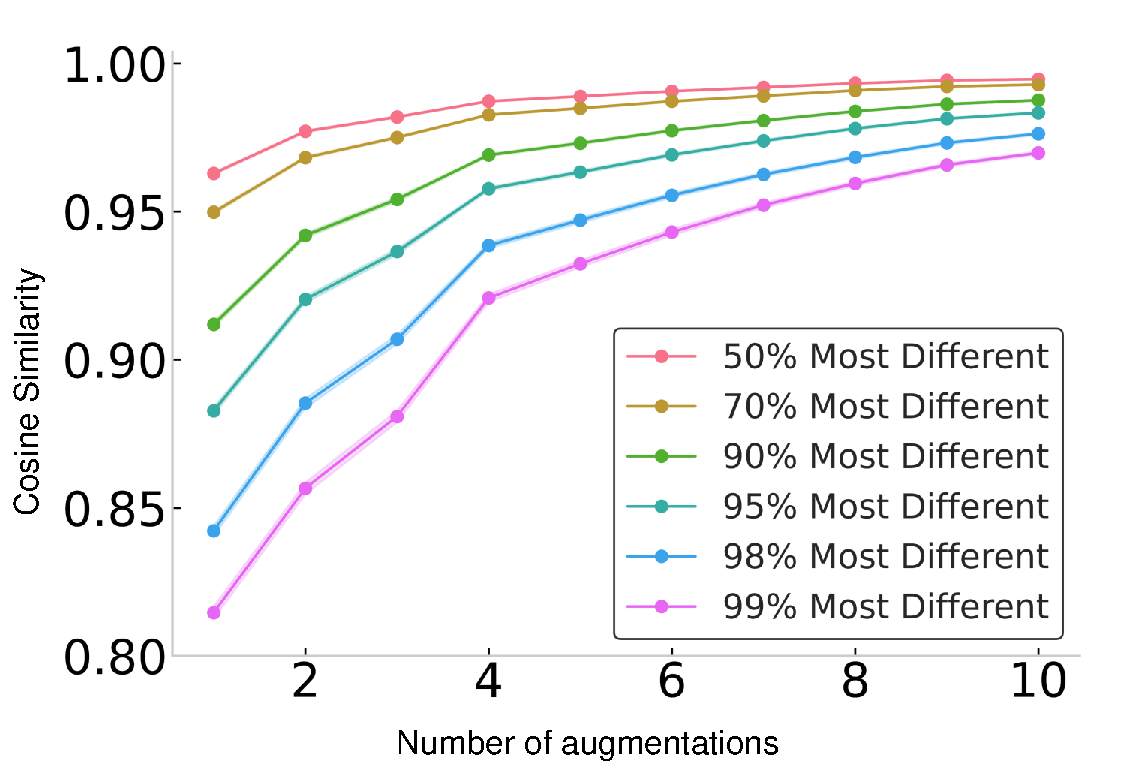
\includegraphics[width=0.98\linewidth]{fig_pdf/num_augmentation.pdf}
    \caption{\textbf{Augmentations improves cosine similarity.} The plot illustrates how increasing the number of augmentations improves the alignment of the model's predictions with the target of 200 augmentations' features, as measured by cosine similarity.}
    \label{fig:ablation_num_of_aug}
  \end{subfigure}
  \hfill
\caption{\textbf{Ablation on number of registers and augmentations} }

\end{figure}

\begin{figure}[t!]
  \centering
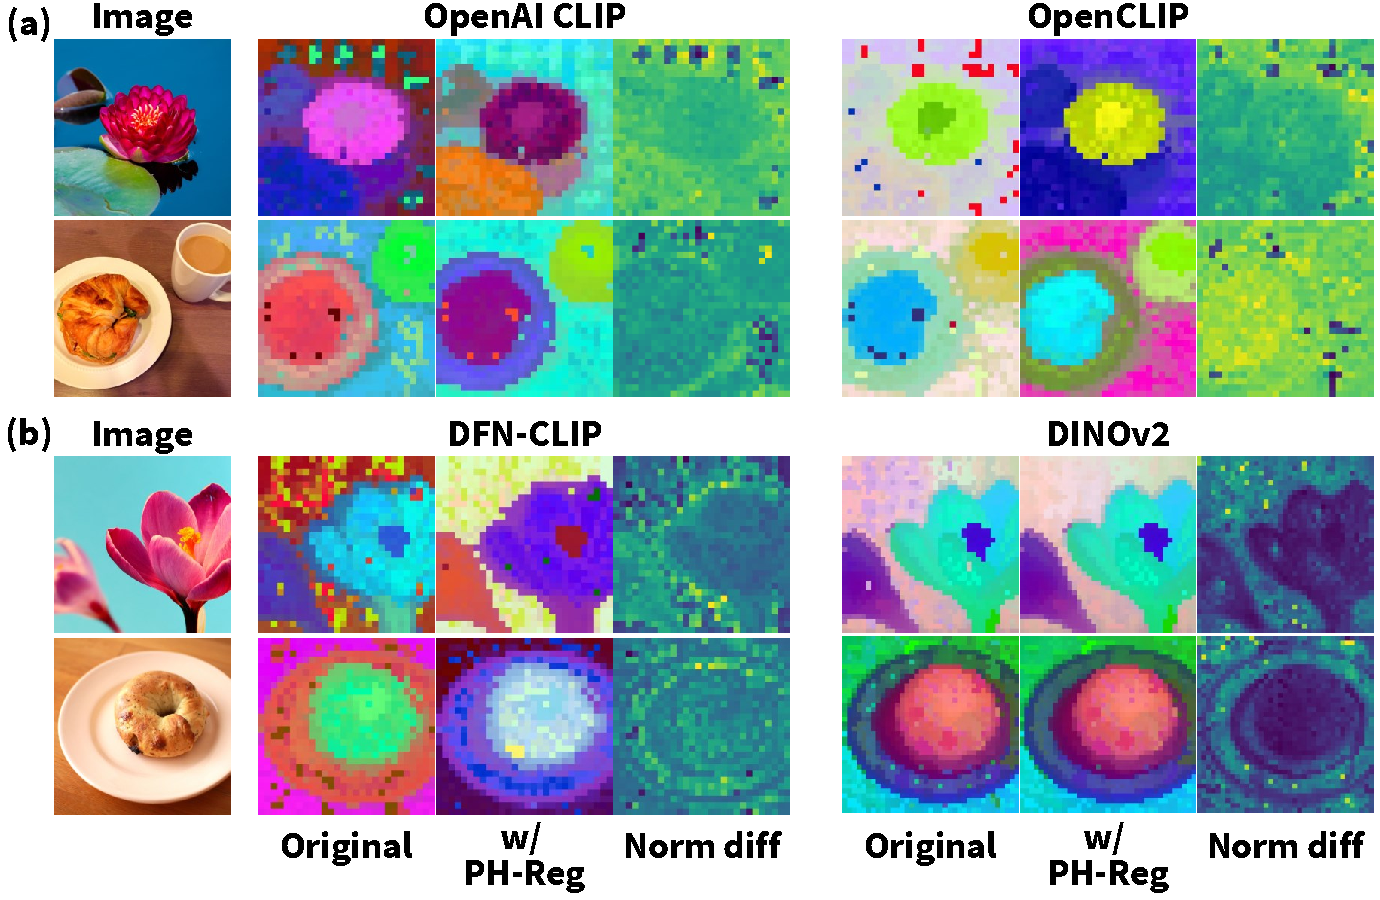
\includegraphics[width=0.8\linewidth]{fig_pdf/norm.pdf}
  \caption{\textbf{Comparison of Original and PH-Reg Features and Norms.} While prior work has noted artifact tokens in DINOv2 as having higher norm than other tokens, we observe this is not the case for all models. Some models have artifact tokens with lower magnitude.}
  \vspace{-0.1cm}
  \label{fig:norms}
\end{figure}
\textbf{The Number of Register Tokens.} We evaluate the influence of the number of register tokens on the cosine similarity between the student model’s outputs and the target values using the COCO Caption dataset~\citep{chen2015microsoft}. Specifically, we distill the student model with 0, 1, 2, 4, 8, or 16 register tokens.

As illustrated in Figure~\ref{fig:ablation_reg}, the cosine similarity increases as the number of register tokens grows, indicating improved alignment with the target representations. However, the performance gain becomes marginal when increasing the number of registers from 4 to 8 and from 8 to 16. Based on this observation, we use 16 register tokens in all subsequent experiments.

\textbf{Distillation Architectural Settings.} We further evaluate the impact of architectural configurations during distillation by analyzing cosine similarity on the COCO Caption dataset. In this setting, we vary the number of register tokens from 0 to 16 while allowing the positional embeddings to be updated during training. As shown in Figure~\ref{fig:ablation_reg}, the improvement in the cosine similarity from unlocking the position embedding becomes less pronounced as the number of register tokens increases. Nonetheless, unlocking positional embeddings continues to provide a positive effect on alignment. This result suggests that in contrast to DVT, the positional embedding itself is unlikely to fully explain the artifact tokens. 

Next, we fix the number of register tokens to 16 and evaluate the effect of unlocking additional layers, including the convolutional patch embedding layer and the later attention layers. For all experiments, we report \textit{50th}, \textit{70th}, \textit{90th}, \textit{95th}, and \textit{99th} percentiles (of cosine similarity to capture the distribution of the most dissimilar features.) Our analysis reveals that incorporating even a single register leads to substantial improvements. In particular, the \textit{99th} percentile of feature cosine similarity in the 1-register configuration exceeds the \textit{50th} percentile (median) of the raw case without registers. This indicates that registers significantly enhance the quality of feature representations across the distribution, not only in extreme cases.

As suggested by~\citep{wang2024sinder,yang2024denoising}, attention layers close to the output also play an important role, which we confirm in our experiments. As shown in Figure~\ref{fig:ablation_reg}, unlocking the last attention layer significantly increases the cosine similarity between the student model's outputs and the target values. While unlocking the convolutional patch embedding layer alone slightly reduces cosine similarity value, the overall value improves when both the convolutional patch embedding and later attention layers are unlocked, compared to the baseline with only unlocked the position embeddings and later attention layers with 16 registers. Therefore, we unlock the positional embeddings, the convolutional patch embedding layer, and the final attention layer during distillation.

\textbf{The Number of Augmentations in the Denoising Process.}
We evaluate our approach using cosine similarity on the COCO Caption dataset to investigate the effect of the number of augmentations. The student model is distilled with 1 to 10 augmentations, where one of them is always an unmodified image.
As shown in Figure~\ref{fig:ablation_num_of_aug}, a high convergence threshold is observed at the \textit{99th} percentile where even the most dissimilar cases exhibit cosine similarity values above 0.95, indicating a substantial reduction in feature space outliers.
As a result, we employ 10 augmentations to generate high-quality features efficiently, thereby reducing computational overhead.

% Please add the following required packages to your document preamble:
% \usepackage{graphicx}
\renewcommand{\arraystretch}{1.2}
\begin{table*}[t]
\centering
\caption{\textbf{Distillation Approaches.} This table reports the contributions of different components in our distillation framework. \textit{Vanilla} refers to the student MaskCLIP, \textit{Denoising Only} refers to MaskCLIP with 10x averaging, the other rows refer to using NACLIP as teacher and MaskCLIP as student.}
\vspace{.1cm}
\resizebox{\columnwidth}{!}{%
\begin{tabular}{l|ccccccccc}
\hline
Approach                       & VOC21 & PC60 & Object & VOC20 & PC59 & Stuff & City & ADE & Avg.            \\ \hline
Vanilla                        & 49.27          & 25.46          & 26.94          & 66.56          & 28.62          & 18.80          & 28.33          & 13.70          & 32.21          \\
Denoising only (10x aug)     & 51.41          & 28.13          & 29.00          & 69.58          & 31.03          & 20.25          & 31.82          & 15.20          & 34.55          \\
Distill, no reg, no denoise & 61.16          & 33.51          & 34.51          & 81.51          & 36.70          & 23.96          & 35.74          & 18.34          & 40.68          \\
Distill, with reg, no denoise  & 61.27          & 33.52          & 34.39          & 81.52          & 36.74          & 23.92          & 35.55          & 18.38          & 40.66          \\
Distill, no reg, with denoise & 62.48          & 34.28          & 35.00          & 82.27          & 37.62          & 24.46          & 36.83          & 18.92          & 41.48          \\
Full Pipeline   & \textbf{63.01} & \textbf{34.52} & \textbf{35.27} & \textbf{83.05} & \textbf{37.88} & \textbf{24.66} & \textbf{37.17} & \textbf{19.22} & \textbf{41.85} \\ \hline
\end{tabular}%
}
\vspace{-.2cm}
\label{tab:ditisll}
\end{table*}
\textbf{Distillation Approaches.} We evaluate the contribution of different components in our distillation approach by conducting open-vocabulary semantic segmentation task on 8 benchmarks. In this setting, the student model is distilled by sequentially removing each component from our approach. These components include the denoising process with 10 augmentations, 16 additional register tokens, and self-distillation.
As shown in Table~\ref{tab:ditisll}, each component contributes to improving the student model's performance. By comparing our full pipeline, where student model is distilled with denoising process and registers, we find that approximately half of the improvement comes from registers, and the other half results from denoising process applied to the teacher model.

% Please add the following required packages to your document preamble:
% \usepackage{graphicx}
\renewcommand{\arraystretch}{1.2}
\begin{table*}[t]
\centering
\caption{\textbf{Effect of Shifting Ratio.} This table reports the impact of different shifting ratios used in the denoising process, as defined in \ref{teacher_method}. Throughout this experiment, we use \texttt{OpenAI CLIP ViT-B/16} as the backbone for the model and apply 10 augmentations in the denosing process.}
\vspace{.1cm}
\resizebox{0.85\columnwidth}{!}{%
\small
\begin{tabular}{l|ccccccccc}
\hline
Ratio & VOC21 & PC60 & Object & VOC20 & PC59 & Stuff & City & ADE & Avg.   \\ \hline
0\%   & 58.88          & 32.20          & 33.15          & 79.70          & 35.16          & 23.30      & 35.48     & 17.42  & 39.41 \\
10\%  & \textbf{60.49} & \textbf{32.91} & \textbf{33.73} & \textbf{80.47} & \textbf{35.94} & 23.86      & 36.60     & 17.94  & 40.24 \\
15\%  & 60.47          & 32.89          & 33.61          & 80.36          & \textbf{35.94}          & \textbf{23.89}      & 36.87     & \textbf{18.10}  & \textbf{40.27} \\
20\%  & 60.39          & 32.82          & 33.46          & 79.93          & 35.85          & 23.86      & 36.98     & 18.07  & 40.17 \\
25\%  & 60.26          & 32.75          & 33.26          & 79.75          & 35.75          & 23.78      & 37.02     & 18.00  & 40.07 \\
30\%  & 60.14          & 32.76          & 33.25          & 79.39          & 35.77          & 23.77      & \textbf{37.07}     & \textbf{18.10}  & 40.03 \\ \hline
\end{tabular}%
}
\label{tab:shift-ratio}
\vspace{-.2cm}
\end{table*}

\textbf{The Ratio of Shifting in the Denoising Process.} To investigate the impact of different shifting ratios in our denoising process, we conduct open-vocabulary semantic segmentation task on 8 benchmarks.
We gradually increase the shifting ratio from 0\% to 30\%, while fixing the number of augmentation at 10. As shown in Table~\ref{tab:shift-ratio}, a shifting ratio of 10\% demonstrates the best performance across 4 datasets, while a shifting ratio of 15\% achieves the best performance across 3 datasets and provides optimal average performance across all 8 datasets. Therefore, we adopt a shifting raio of 15\% in denoising process when applied to the teacher model.

\subsection{Investigation of Artifacts and Registers}
While prior work has noted that artifact tokens are high magnitude in DINOv2~\cite{darcet2023vision}, in Figure~\ref{fig:norms} we find that this is not always the case. In OpenAI CLIP and OpenCLIP, the artifacts are generally lower norm than their surrounding patches. In contrast, in DFN-CLIP and DINOv2, the artifacts are higher norm. This illustrates that there may be elements of the training dynamic at play, as the artifact norms can differ even when the training objective is very similar. In Figure~\ref{fig:visualization_norm} we visualize the norms of the original network and those with registers added, we find that our method effectively reduces the variance of the patch norms. 